\documentclass[12pt,letterpaper]{article}
\usepackage{pdfpages}
\usepackage{fancyhdr}
\usepackage[colorlinks=true, urlcolor=blue, linkcolor=blue]{hyperref}
\usepackage{graphicx}
\usepackage[top=1.4in, left=0.5in, right=0.5in, bottom=0.8in]{geometry}
\usepackage[T1]{fontenc}
\usepackage{helvet}
\pagestyle{fancy}
\renewcommand{\headrulewidth}{0pt}
\renewcommand{\footrulewidth}{0pt}
\setlength{\parindent}{0em}
\setlength{\parskip}{1em}


\fancyfoot[C]{\setlength{\unitlength}{1in}\begin{picture}(5,0)\put(-1.8,-1){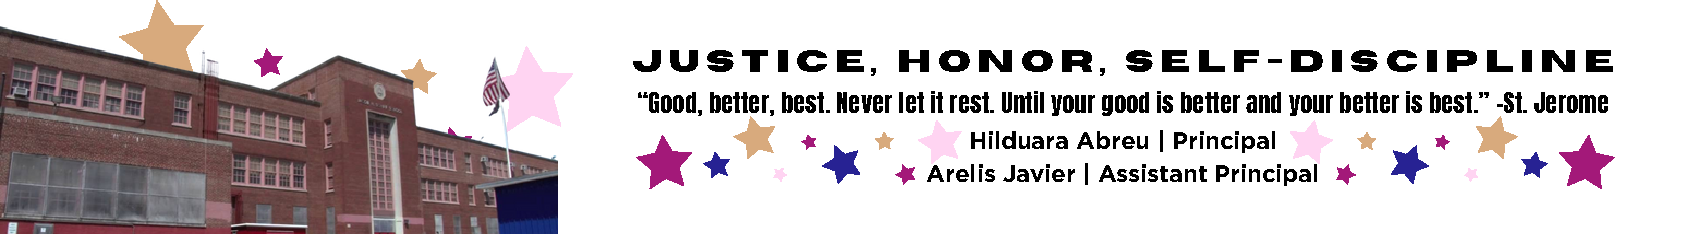
\includegraphics[width=8.8in,height=1.3in]{logo-1}}\end{picture}}
\fancyhead[C]{\setlength{\unitlength}{1in}\begin{picture}(5,0)\put(-1.9,-1){
\includegraphics[width=8.9in,height=1.3in]{logo-2}}\end{picture}}

\pagenumbering{gobble}
\addtolength{\evensidemargin}{-2in}
\addtolength{\topmargin}{-0.5in}
\addtolength{\textwidth}{0in}
%%%%%%%%%%%%%%%%%%%%%%%%%%%%%%%%%%%%%%%%%%%%%%%%%%%%%%%%%%%%%%%%%%

\begin{document}
\vspace*{0.5in}
Date: \href{https://www.ps192.org/apps/bbmessages/show_bbm.jsp?REC_ID=139439}{September 14, 2023} 

\textbf{Subject: Welcome letter to our new school year 2023-24}

Dear P.S. 192 Families Grades K-5,

As we approach the commencement of the new school year for 2023-24, commencing on 
September 7th, we extend a warm welcome to all our students. We trust that you have had a
pleasant and healthy summer break. Our devoted and compassionate team of educators and
school personnel eagerly anticipates your return for what promises to be a year filled
with excitement, laughter and learning.

As we gear up for your child's return, we want to share important information in place at
P.S. 192 to ensure a safe and enjoyable learning experience for everyone. Please take note
of the following guidelines:
	\begin{itemize}
	\item Uniforms: All students are required to come to school daily dressed in their
	uniforms, which remain the same: a burgundy shirt and navy bottoms (pants, skirt, 
	jumper).
	\item Arrival and Dismissal: To ensure a safe and efficient arrival and dismissal 
	process, please take note of the following schedule. There will be staff members and 
	signs pointing families to where to go during the first week of school.
	\item Arrival: New this year, ALL students in Grades K-5 will enter through the 
	Cafeteria each morning, beginning at 7:40 AM to eat breakfast.
	\item Dismissal: New this year, ALL students in Grades K-5 will be dismissed from the
	backyard at 2:15 PM. There will be designated spots for each class by grade. Please
	follow the signs.
	\item School Supplies: PS 192 will be providing all basic school supplies, such as
	notebooks, folders, and crayons. We only ask that families in Grades K-5 provide
	students with a backpack and one box of Ziplock gallon-size bags for students to use
	for centers, book baggies and math tool kits. object like a doll or stuffed animal.
	\end{itemize}

We feel privileged to be part of a community where parents, teachers, staff, and students
work together to build strong relationships that support academic and social growth. We
are eagerly looking forward to your participation in the various events throughout the
school year and welcome your active involvement in your child's educational journey.
\pagebreak
\vspace*{2cm}
It is an honor to be part of a community where parents, teachers, staff, and students
collectively strive to foster strong relationships that promote academic and social growth. We eagerly anticipate your participation in the events scheduled throughout the
school year and value your active engagement in your child's education.

Regular updates regarding your child's school-wide events will be communicated through Our
Website: \url{www.ps192.org}, \href{https://www.classdojo.com/}{ClassDojo}, School Messenger, and our WhatsApp group. Should you have any questions, please do not hesitate to contact our Parent Coordinator, Angela Rijo,at \url{www.ps192.org/angela}, or (646) 745-0150.

We will be hosting events throughout the year and look forward to partnering with you both
in person and virtually. Please stay tuned for more information on all of our upcoming
events:
	\begin{itemize}
	\item On September 14th, we will be hosting our first Virtual \href{https://www.ps192.org/apps/pages/index.jsp?uREC_ID=1504975&type=d&pREC_ID=2510452&tota11y=true}{Meet and Greet} from 4:30-7:30 PM to meet your child’s teacher.
	\item On September 28th, we will be hosting our first Coffee with the Principal in
	person at 8:00 AM.
	\end{itemize}
 
We are eagerly counting down the days until we can welcome you back on Thursday, September 7th. I am honored to serve as the principal of PS 192, and I extend my heartfelt gratitude
for your cooperation and dedication to the well-being of our children, staff, and school.

Warmest regards,


\includegraphics[width=0.2\textwidth]{hil_signature}

\textbf{Principal P.S. 192}

\textit{The School of Joyful Learning!}

\url{www.ps192.org}

\end{document}
